
%(BEGIN_QUESTION)
% Copyright 2003, Tony R. Kuphaldt, released under the Creative Commons Attribution License (v 1.0)
% This means you may do almost anything with this work of mine, so long as you give me proper credit

Complete this table, performing all necessary conversions between numeration systems on these fixed-point number values.  Truncate all answers to three characters past the point:

$$\includegraphics[width=15.5cm]{i02170x01.eps}$$

\underbar{file i02170}
%(END_QUESTION)





%(BEGIN_ANSWER)

$$\includegraphics[width=15.5cm]{i02170x02.eps}$$

%(END_ANSWER)





%(BEGIN_NOTES)

Lots of conversions to do here!  I particularly like the ``table'' format shown here for practicing numeration system conversions, because it compresses a lot of practice into a small space on paper, and also because it allows students to use different methods of conversion.  For example, in converting a decimal number to the other forms, a student might choose to convert first to binary, then from binary to octal and hex.  Or, alternatively, a student may choose to convert from decimal into hex, then from hex into binary, then from binary to octal, the last two conversions being especially easy.

%INDEX% Electronics review: numeration system conversions

%(END_NOTES)


